\section{Wellen}
\begin{itemize}
    \setlength\itemsep{1pt}
    \item raumzeitlicher Vorgang $cos(\omega t- \beta z)$
    \item Energie- ohne Materietransport
    \item Poyntingvektor $\vec{S}=\vec{E}\times\vec{H} \left[ \dfrac{W}{m^2} \right]$\\
        {\footnotesize Falls $\vec{E}\perp\vec{H}$ und $\vec{S}\perp\vec{E}$ und $\vec{S}\perp\vec{H}$}
\end{itemize}

\subsubsection*{Wellengleichung}
\underline{Tatsächlicher Zeitverlauf}(Realteil von $\underline{\vec{E}}(z,t)$)
\begin{empheq}[]{align*}
    \vec{E}(z,t)
    = E_0
    \cdot \overbrace{e^{-\alpha z}}^{\mathclap{\text{Dämpfung}}}
    \cdot \underbrace{cos(\omega t \overbrace{-}^{\mathclap{\text{positive z-Richtung}}} \beta z)}_\text{Zeit- \& Raumausb. (Wellenz./S)}
    \cdot \overbrace{\vec{e}_z}^{\mathclap{\text{Feldausb.}}}
\end{empheq}
\underline{Komplexer Amplitudenvektor}
\begin{empheq}[]{align*}
    \boxed{\underline{\vec{E}}(z,t)
        = E_0\cdot e^{-\alpha z}\cdot e^{j(\omega t-\beta z)}\cdot\vec{e}_z
        = E_0\cdot e^{-\underline{\gamma}z}\cdot e^{j\omega t}\cdot\vec{e}_z
    }
\end{empheq}

\underline{Fortpflanzungskonstante $\gamma$}
\[\boxed{\underline{\gamma}=\alpha+j\beta}\]

$\alpha$ : Dämpfungskonstante [Np/m]

$\beta$ : Phasenkonstante [rad/m]

$v_p$ : Phasengeschwindigkeit [m/s] $\left(= \sqrt{x^2 + y^2 \dots} \right)$

$v_g$ : Gruppengeschwindigkeit [m/s]

\subsection{Grundlagen}
\textbf{Brechungszahl:}
\[ n = \dfrac{c_0}{c} = \sqrt{\epsilon_r} \geq 1 \]

\textbf{Wellenzahl:}
Im Vakuum: $k_{0}=\frac{\omega}{c_{0}}$
\begin{align*}
    \beta & = \frac{\omega}{v_p} = \frac{2 \pi f}{v_p} = |\vec{\beta}|                                                                      \\
      & = \frac{\omega \cdot n}{c_{0}} = n \cdot k_{0}=\frac{1}{\sqrt{\mu_{r} \cdot \varepsilon_{r}}} \cdot k_{0}=k_{r} \cdot k_{0}
\end{align*}

\textbf{Wellenlänge:}
\begin{align*}
    \lambda   & = \dfrac{\lambda_0}{\sqrt{\mu_r \cdot \varepsilon_r}} = \dfrac{2 \pi}{\beta} = \dfrac{v_p}{f} = [m] \\
              & = \dfrac{\lambda_0}{n} = \dfrac{2 \pi}{n \cdot k_0}                                             \\
    \lambda_0 & = \dfrac{c_0}{f} = \dfrac{2\pi}{k_0}
\end{align*}

\textbf{Phasengeschwindigkeit:}
\[
    v_p = \dfrac{\omega}{\beta} = \frac{c_0}{\sqrt{ \mu_r \varepsilon_r }}  = \frac{1}{\sqrt{ \mu_r \mu_0 \varepsilon_r \varepsilon_0}} \qquad v_{p,\texttt{Medium} \leq c_0}
\]


\subsection{Ausbreitung}
\subsubsection{Allgemein}
\begin{align*}
    \lambda                 & = \dfrac{2\pi}{\beta} \qquad E_2 = E_1 e^{-\alpha z}                                                                                        \\
    v_p                     & = \lambda\cdot f = \dfrac{\omega}{\beta}                                                                                                    \\
    \alpha                  & = \omega \cdot \sqrt{\dfrac{\mu \varepsilon}{2}\cdot \left(\sqrt{1+\dfrac{\kappa^2}{\omega^2\cdot\varepsilon^2}} - 1\right)}   \\
    \beta                   & = \omega \cdot \sqrt{\dfrac{\mu \varepsilon}{2}\cdot \left(\sqrt{1+\dfrac{\kappa^2}{\omega^2\cdot\varepsilon^2}} + 1\right)} \\
    \Aboxed{\underline{Z}_F & = \dfrac{\underline{E}}{\underline{H}} = \sqrt{\dfrac{j\omega\mu}{\kappa+j\omega\varepsilon}} = \dfrac{1}{n}\sqrt{\dfrac{\mu_0}{\varepsilon_0}} = Z_{F0} \cdot \sqrt{\dfrac{\mu_r}{\varepsilon_r }}}                                              \\
\end{align*}

\subsubsection{Im leeren Raum(Vakuum)}
\begin{align*}
    \alpha                     & = 0                                                                    \\
    \beta                          & = \dfrac{\omega}{c_0}                                                  \\
    \lambda                    & = \dfrac{c_0}{f}                                                       \\
    v_p                        & = c_0                                                                  \\
    \Aboxed{\underline{Z}_{F0} & = \sqrt{\dfrac{\mu_0}{\varepsilon_0}} = 120 \pi\Omega\approx377\Omega}
\end{align*}

\subsubsection{Im verlustlosen/idealen Dielektrika}
verlustlos: $\kappa =0$, maximale Wirkleistung

$Z_F$ rein reel $\rightarrow$ ebene Welle
\begin{align*}
    \alpha                  & = 0                                                                                              \\
    \beta                       & = \dfrac{\omega}{c_0}\sqrt{\mu_r\varepsilon_r}=\omega\sqrt{\mu\varepsilon}=\dfrac{2\pi}{\lambda} \\
    \lambda                 & = \dfrac{c_0}{f}\dfrac{1}{\sqrt{\mu_r\varepsilon_r}}                                             \\
    v_p                     & = \dfrac{c_0}{\sqrt{\mu_r\varepsilon_r}}                                                         \\
    \Aboxed{\underline{Z}_F & = \sqrt{\dfrac{\mu}{\varepsilon}}}
\end{align*}

\subsubsection{Im Dielektrika mit geringem Verlust}
geringer Verlust: $\dfrac{\kappa}{\omega\varepsilon} \ll 1$

\begin{align*}
    \alpha                  & \approx\dfrac{\kappa}{2}\cdot\sqrt{\dfrac{\mu}{\varepsilon}} = \frac{\kappa}{2}\cdot Z_{F0}                                                                \\
    \beta                   & \approx\omega\sqrt{\mu\varepsilon}\left(1+\dfrac{1}{8}\cdot\dfrac{\kappa^2}{\omega^2\varepsilon^2}\right)                                                  \\
    \lambda                 & = \dfrac{c_0}{f}\cdot\dfrac{1}{\sqrt{\mu_r\varepsilon_r}}\cdot\frac{1}{1+\frac{1}{8}\left(\frac{\kappa}{\omega\varepsilon}\right)^2}                       \\
    v_p                     & = \dfrac{c_0}{\sqrt{\mu_r\varepsilon_r}}\cdot\frac{1}{1+\frac{1}{8}\left(\frac{\kappa}{\omega\varepsilon}\right)^2}                                        \\
    \Aboxed{\underline{Z}_F & = \sqrt{\dfrac{\mu}{\varepsilon}}\left(1-\frac{j\kappa}{\omega\varepsilon}\right)^{-^1/2} \approx Z_{F0}\left(1+\frac{j\kappa}{2\omega\varepsilon}\right)}
\end{align*}

\subsubsection{Im guten Leiter}
geringer Verlust: $\dfrac{\kappa}{\omega\varepsilon} \gg 1$
\begin{align*}
    \alpha                  & \approx \beta \approx\sqrt{\frac{\omega\mu\kappa}{2}}=\dfrac{1}{\delta}\sim\sqrt{f} \\
    \lambda                 & = 2\pi \sqrt{\dfrac{2}{\omega\mu\kappa}}=2\pi\delta                                 \\
    v_p                     & = \frac{2\pi}{\beta} = \omega\delta                                                 \\
    \Aboxed{\underline{Z}_F & = \sqrt{\dfrac{j\omega\mu}{\kappa}} \approx \dfrac{1+j}{\kappa\cdot\delta}}
\end{align*}
\newpage
\subsection{Übergang}
\subsubsection{Zwischen Dielektrika mit geringem Verlust}

% \input{Figures/Wellen_Uebergang_mit_geringem_Verlust.tex}
% 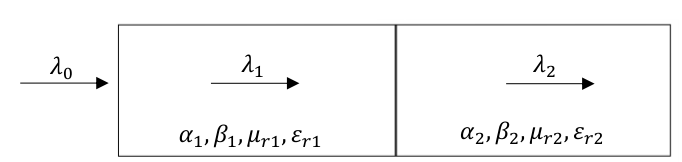
\includegraphics[width=\columnwidth]{Figures/UebergangzweiDielektrika.png}
\begin{align*}
    \lambda_1 & = \dfrac{\lambda_0}{\sqrt{\mu_{r1}\varepsilon_{r1}}}          & \lambda_2 & = \dfrac{\lambda_0}{\sqrt{\mu_{r2}\varepsilon_{r2}}}                                     \\
    \beta_1   & = \dfrac{2\pi}{\lambda_0}\cdot\sqrt{\mu_{r1}\varepsilon_{r1}} & \beta_2   & = \dfrac{2\pi}{\lambda_0}\cdot\sqrt{\mu_{r2}\varepsilon_{r2}}                            \\
    Z_{F1}    & = \dfrac{Z_{F0}}{\sqrt{\mu_{r1}\varepsilon_{r1}}}             & Z_{F2}    & = \dfrac{Z_{F0}}{\sqrt{\mu_{r2}\varepsilon_{r2}}}
\end{align*}

\subsection{Energie und Poyntingvektor (Energieflussdichte)}
\begin{align*}
    \vec{S}             & =  \vec{E}\times\vec{H} = E_{eff} H_{eff} \qquad \si{\left[\frac{W}{m^2}\right]} \\
    \vec{S}_{\text{av}} & =  \frac{1}{2} \cdot Re\{\vec{E}\times\vec{H}^*\}              \\
    S_{AV}              & =  \frac{1}{2} \cdot \hat{E} \cdot \hat{H} = \frac{1}{2} \cdot \dfrac{E^2}{Z_{F0}} = \\
                        & =  \frac{1}{2} \cdot H^2 \cdot Z_{F0} =  \dfrac{P}{A_\texttt{Fläche}}                                \\
\end{align*}

\subsubsection{An Grenzflächen}
\begin{align*}
    S_t &= S_h - S_r \\
    S_t &= S_h  (1 - r_e^2) \cdot \frac{\cos \alpha_1}{\cos \alpha_2}
\end{align*}

\subsubsection{Leistung}
\begin{align*}
    P     & = \iint\vec{S}_{\text{av}}d\vec{a}                   \\
          & = Re\left\{\underline{U}\cdot\underline{I}^*\right\} \\
    P_1   & = P_0 \cdot e^{-2\alpha z}                           \\
    W_{M} & = 1/_2\cdot\mu\cdot H^2                              \\
    W_{E} & = 1/_2\cdot\varepsilon\cdot E^2
\end{align*}

\subsubsection{Leistung vom Kabel transportiert}

\begin{align*}
    P & = \dfrac{\hat{U}^2}{2\cdot Z_L}
\end{align*}

\subsection{dÀlembertsche Gleichung (allg.)}
\begin{align*}
    \Delta \vec{E}-\kappa \mu \frac{\partial \vec{E}}{\partial t}-\varepsilon \mu \frac{\partial^{2} \vec{E}}{\partial t^{2}} & = \operatorname{grad} \frac{\rho}{\varepsilon} \\
    \Delta \vec{H}-\kappa \mu \frac{\partial \vec{H}}{\partial t}-\varepsilon \mu \frac{\partial^{2} \vec{H}}{\partial t^{2}} & = 0
\end{align*}

Isolator, ideales Dielektrikum, Nichtleiter $\kappa = 0$
\begin{align*}
    \Delta \vec{E} & =\varepsilon \mu \frac{\partial^{2} \vec{E}}{\partial t^{2}}+\operatorname{grad} \frac{\rho}{\varepsilon} \\
    \Delta \vec{H} & =\varepsilon \mu \frac{\partial^{2} \vec{H}}{\partial t^{2}}
\end{align*}

sehr gute Leiter
\begin{align*}
    \Delta \vec{E} & =\kappa \mu \frac{\partial \vec{E}}{\partial t}+\operatorname{grad} \frac{\rho}{\varepsilon} \\
    \Delta \vec{H} & =\kappa \mu \frac{\partial \vec{H}}{\partial t}
\end{align*}

\subsection{Helmholtz-Gleichungen (Frequenzbereich)}
\begin{align*}
    \Delta \underline{\vec{E}}-\left(\kappa \mu \cdot \mathrm{j} \omega-\varepsilon \mu \cdot \omega^{2}\right) \cdot \underline{\vec{E}} & = \operatorname{grad} \frac{\rho}{\varepsilon} \\
    \Delta \underline{\vec{H}}-\left(\kappa \mu \cdot \mathrm{j} \omega-\varepsilon \mu \cdot \omega^{2}\right) \cdot \underline{\vec{H}} & = 0
\end{align*}

\subsubsection{Zeitbereich}
\begin{align*}
    \Delta \vec{E}-\varepsilon \mu \frac{\partial^{2} \vec{E}}{\partial t^{2}} & =0 \\
    \Delta \vec{H}-\varepsilon \mu \frac{\partial^{2} \vec{H}}{\partial t^{2}} & =0
\end{align*}

\subsubsection{Frequenzbereich (harmonisch)}
\begin{align*}
    \Delta \underline{\vec{E}}+\varepsilon \mu \omega^{2} \cdot \underline{\vec{E}} & =0 \\
    \Delta \underline{\vec{H}}+\varepsilon \mu \omega^{2} \cdot \underline{\vec{H}} & =0
\end{align*}

\textbf{Zeitabhängigkeit harmonisch:}
\begin{align*}
    \Delta \vec{H}   & = (j \omega \mu \kappa - \omega^2 \varepsilon \mu ) \vec{H}                                  \\
    \Delta \vec{E} i & = (j \omega \mu \kappa - \omega^2 \varepsilon \mu ) \vec{E} + grad \frac{ \rho}{\varepsilon}
\end{align*}

\textbf{keine Raumladung $ \rho = 0$}
\begin{align*}
    \Delta \vec{E} & = (j \omega \mu \kappa - \omega^2 \varepsilon \mu ) \vec{E}
\end{align*}

\textbf{Ebene Wellen}
\begin{align*}
    \Delta \vec{E} & = \frac{ \partial \vec{E}}{ \partial z^2} = j \omega \mu ( \kappa + j \omega \varepsilon) \vec{E} \\
    \Delta \vec{H} & = \frac{ \partial \vec{E}}{ \partial z^2} = j \omega \mu ( \kappa + j \omega \varepsilon) \vec{H}
\end{align*}

%%%%%%%%%%%%%%%%%

\subsubsection{Gruppengeschwindigkeit}
\begin{align*}   
    v_g        &= \dfrac{d \omega}{d k} = \dfrac{\textnormal{Wegstück der Wellengruppe}}{\textnormal{Laufzeit der Wellengruppe}}    \\                                                                                                                                                                                     \\
    E(z,t)     & = 2E\cdot\underbrace{\cos(\omega_0t-\beta_0z)}_{\mathclap{\text{Grundfrequenz $\omega$}}}\cdot\underbrace{\cos(\Delta\omega t-\Delta\beta z)}_{\mathclap{\text{Einhüllende $\Delta\omega$}}} \\
    v_p        & = \frac{\omega_0}{\beta_0}                                                                                                                                                                   \\
    v_g        & = \frac{\Delta\omega}{\Delta\beta}
\end{align*}

\subsection{Polarisation}
\begin{tabularx}{0.45\textwidth}{>{\hsize=.27\hsize}X|>{\hsize=.5\hsize}X|>{\hsize=.23\hsize}X}
    Lineare      & wenn der Endpunkt des E–Vektors eine Linie beschreibt & $H$ oder $E$ \\
    \hline
    Elliptische  & Endpunkt des E-Vektors eine Ellipse beschreibt        & $E\neq H$    \\
    \hline
    Kreisförmige & der Endpunkt des E-Vektors einen Kreis beschreibt     & $E = H$      \\
\end{tabularx}

% \subsection{Verlustlose Polarisation}
% \begin{align*}
%     Z_F & = \sqrt{\frac{\mu}{\varepsilon}}                                                                                                                                             \\
%     r_s & = \frac{\sqrt{\varepsilon_{r1}}\cdot\cos\theta_i - \sqrt{\varepsilon_{r2}}\cdot\cos\theta_t}{\sqrt{\varepsilon_{r2}}\cdot\cos\theta_t + \sqrt{\varepsilon_{r1}}\cos\theta_i} \\
%     t_s & = \frac{2\cdot\sqrt{\varepsilon_{r1}}\cdot\cos\theta_i}{\sqrt{\varepsilon_{r2}}\cdot\cos\theta_t + \sqrt{\varepsilon_{r1}}\cdot\cos\theta_i}                                 \\
%     r_p & = \frac{\sqrt{\varepsilon_{r1}}\cdot\cos\theta_t - \sqrt{\varepsilon_{r2}}\cdot\cos\theta_i}{\sqrt{\varepsilon_{r2}}\cdot\cos\theta_i + \sqrt{\varepsilon_{r1}}\cos\theta_t} \\
%     t_p & = \frac{2\cdot\sqrt{\varepsilon_{r1}}\cdot\cos\theta_i}{\sqrt{\varepsilon_{r2}}\cdot\cos\theta_i + \sqrt{\varepsilon_{r1}}\cdot\cos\theta_t}
% \end{align*}

\subsection{Totalrefexion, Grenzwinkel}
\begin{align*}
    \sin\alpha_g & = \frac{n_2}{n_1} = \sqrt{ \frac{\varepsilon_{r2}\mu_{r2}}{\varepsilon_{r1}\mu_{r1}}}\\
    \alpha_g & = \sin^{-1} \left( \sqrt{ \dfrac{\mu_{r2} \varepsilon_{r2}}{\mu_{r1} \varepsilon_{r1}}} \right)\\
    \dfrac{\sin \alpha_{2}}{\sin \alpha_{1}} = \dfrac{k_{h}}{k_{g}} & = \sqrt{\dfrac{\mu_{r 1} \varepsilon_{r 1}}{\mu_{r 2} \varepsilon_{r 2}}} = \dfrac{n_{1}}{n_{2}} = \dfrac{v_{p, 2}}{v_{p, 1}} = \dfrac{\lambda_{2}}{\lambda_{1}} \\
\end{align*}

\subsection{Stehwellenverhältnis}
\[
    \mathrm{SWR} = \frac{E_{\max}}{E_{\min}}=\frac{H_{\max}}{H_{\min}}=\frac{E_{h}+E_{r}}{E_{h}-E_{r}} = \frac{1+|r|}{1-|r|} \quad 1<s<\infty
\]

\subsection[Senkrechter Einfall]{Senkrechter Einfall $ \theta_h = 0$ }

\input{Figures/Wellen_Senkrechter_Uebergang.tex}

\begin{align*}
    r  &= r_e = r_m\frac{Z_{F2} - Z_{F1}}{Z_{F1} + Z_{F2}} = \frac{n_2 - n_1}{n_1 + n_2}\\
    n &= \sqrt{\epsilon_r \cdot \mu_r} \\
    0<t&<2 \qquad 0<|r|<1
\end{align*}

Elektrisches Feld:   
\begin{align*}
    E_t &= t_e \cdot E_h \qquad E_r = r_e \cdot E_h
    %\vec{E_t}    & = \vec{E_h} + \vec{E_r} \\
    E_t          & = E_h + E_r             \\
    t_e\cdot E_{h} & = E_{h} + r_e\cdot  E_{h} \\
    t_e            & = 1+ r_e = \dfrac{2 \cdot n_2}{n_1 + n_2}
\end{align*}

Magnetisches Feld:
\begin{align*}
    H_t &= t_m \cdot H_h \qquad H_r = r_m \cdot H_h     	                            \\
    % \vec{H_t}                   & = \vec{H_h}-\vec{H_r}                                \\
    H_t                         & = H_h - H_r                                           \\
    % \frac{t_m\cdot E_{h}}{Z_{F2}} & = \frac{E_{h}}{Z_{F1}} - \frac{r_m\cdot E_{h}}{Z_{F1}} \\
    \frac{t_m}{Z_{F2}}            & = \frac{1}{Z_{F1}} - \frac{r_m}{Z_{F1}}             \\
    t_m &= \dfrac{2 \cdot n_1}{n_1 + n_2}                                               \\
    r_m &= \dfrac{n_2 - n_1}{n_1 + n_2}
\end{align*}




\subsubsection[Senkrechter Einfall ideales/verlustl. Dielekt.]{Senkrechter Einfall ideales/verlustl. Dielekt. $\kappa = 0$}

%\includegraphics[width=\columnwidth]{Figures/senkrechterEinfall.png}

\begin{align*}
    \text{reel: }Z_F          & = \sqrt{\frac{\mu}{\varepsilon}} \\
    \texttt{imaginär: }\gamma & = j \omega\sqrt{\mu\varepsilon}
    r = \frac{Z_{F2} - Z_{F1}}{Z_{F1} + Z_{F2}} &= \frac{\sqrt{\frac{\mu_2}{\varepsilon_2}} - \sqrt{\frac{\mu_1}{\varepsilon_1}}}{\sqrt{\frac{\mu_2}{\varepsilon_2}} + \sqrt{\frac{\mu_1}{\varepsilon_1}}} \\
    t = \frac{2 Z_{F2}}{Z_{F1} + Z_{F2}} &= \frac{2\sqrt{\varepsilon_{r1}\mu_{r2}}}{\sqrt{\varepsilon_{r1}\mu_{r2}}+\sqrt{\varepsilon_{r2}\mu_{r1}}}
\end{align*}

% \begin{tabularx}{\columnwidth}{>{\hsize=.35\hsize}X|>{\hsize=.32\hsize}X>{\hsize=.18\hsize}X>{\hsize=.18\hsize}X}
%     idealer Leiter    & $ Z_{F2} = 0 $                    & $ r = -1 $ & $t = 0$ \\
%     \hline
%     ideales Dielektr. & $\mu_{r1} = \varepsilon_{r1} = 1$ &            &         \\
% \end{tabularx}

% \subsubsection[Spezialfall Medium 1 ist Luft]{Spezialfall $\underline{Medium 1}$ ist Luft}
% \begin{align*}
%     \Aboxed{ & \mu_{r1} = \varepsilon_{r1} = 1}                                                            \\
%     r        & = \frac{\sqrt{\mu_{r2}}-\sqrt{\varepsilon_{r2}}}{{\sqrt{\mu_{r2}}+\sqrt{\varepsilon_{r2}}}} \\
%     t        & = \frac{2\sqrt{\mu_{r2}}}{\sqrt{\mu_{r2}}+\sqrt{\varepsilon_{r2}}}
% \end{align*}

% \subsubsection[Spezialfall Medium 2 ist Luft]{Spezialfall $\underline{Medium 2}$ ist Luft}
% \begin{align*}
%     \Aboxed{ & \mu_{r2} = \varepsilon_{r2} = 1}                                                            \\
%     r        & = \frac{\sqrt{\varepsilon_{r1}}-\sqrt{\mu_{r1}}}{{\sqrt{\varepsilon_{r1}}+\sqrt{\mu_{r1}}}} \\
%     t        & = \frac{2\sqrt{\varepsilon_{r1}}}{\sqrt{\mu_{r1}}+\sqrt{\varepsilon_{r1}}}
% \end{align*}

\subsubsection[Spezialfall beide Medien NICHT magnetisch]{Spezialfall $\underline{beide Medien}$ NICHT magnetisch}
\begin{align*}
    \Aboxed{ & \mu_{r1} = \mu_{r2} = 1}                                                                                    \\
    r        & = \frac{\sqrt{\varepsilon_{r2}}-\sqrt{\varepsilon_{r1}}}{{\sqrt{\varepsilon_{r1}}+\sqrt{\varepsilon_{r2}}}} \\
    t_m      & = \frac{2\sqrt{\varepsilon_{r1}}}{\sqrt{\varepsilon_{r1}}+\sqrt{\varepsilon_{r2}}}
\end{align*}

\subsubsection[Spezialfall Medium 2 idealer Leiter]{Spezialfall $\underline{Medium 2}$ idealer Leiter}
\begin{align*}
    Z_{F2}       & = 0                                 \\
    r            & = -1                                \\
    t            & = 0                                 \\
    \overline{S} & = 0                                 \\
    E_1          & = -2j\cdot E_h\cdot \sin(\beta_1 z) \\
    H_1          & = 2\cdot H_h\cdot \cos(\beta_1 z)
\end{align*}
\begin{align*}
     & \underline{Stehende Welle}                                              \\
     & \rightarrow \text{$H_{max}$ und $E_{min}$ bei } n \cdot \lambda/_2      \\
     & \rightarrow \text{$H_{min}$ und $E_{max}$ bei } (2n-1) \cdot \lambda/_4 \\
     & \qquad \rightarrow 90^\circ Phasenverschiebung
\end{align*}

\newpage
\subsection{Senkrechte (E-Feld) Polarisation (H-Feld parallel)}
\input{Figures/SchraegerUebergang_senk_Polarisation.tex}

\begin{flalign*}
	Z_{F(n)}                & = Z_{F0}\cdot\sqrt{\frac{\mu_{r(n)}}{\varepsilon_{r(n)}}}&
	\frac{Z_{F1}}{Z_{F2}} & = \frac{\sqrt{\mu_{r 1}\varepsilon_{r2}}}{\sqrt{\mu_{r 2}\varepsilon_{r1}}}&
\end{flalign*}

\textbf{Brechungsgesetz}: \qquad  mit $ \theta_h = \theta_r\ $
\begin{flalign*}
	\Aboxed{\frac{\sin\theta_t}{\sin\theta_h} & = \sqrt{\frac{\mu_{r 1}\varepsilon_{r1}}{\mu_{r 2}\varepsilon_{r2}}}} = \frac{\lambda_2}{\lambda_1}= \frac{\beta_1}{\beta_2}= \frac{n_1}{n_2} &
\end{flalign*}

\textbf{Fresnelsche Formeln ohne $\mu_r$}
\begin{flalign*}
		    r_s    & =  r_{es} = r_{ms} =                                                                                                                                            \\
		& = \frac{Z_{F2} \cdot \cos \theta_h-Z_{F1} \cdot \cos \theta_t}{Z_{F2} \cdot \cos \theta_h+Z_{F1} \cdot \cos \theta_t}                                           
%		& = \frac{\cos\theta_h-\sqrt{^{\varepsilon_{r2}}/_{\varepsilon_{r1}}-\sin^2\theta_h}}{\cos\theta_h+\sqrt{^{\varepsilon_{r2}}/_{\varepsilon_{r1}}-\sin^2\theta_h}} \\
		= \frac{\sqrt{\varepsilon_{r1}}\cdot\cos\theta_h - \sqrt{\varepsilon_{r2}}\cdot\cos\theta_t}{\sqrt{\varepsilon_{r2}}\cdot\cos\theta_t + \sqrt{\varepsilon_{r1}}\cos\theta_h} \\
		& = \frac{\cos \theta_h-\sqrt{\frac{\varepsilon_{r 2}}{\varepsilon_{r 1}}-\sin ^2 \theta_h}}{\cos \theta_h+\sqrt{\frac{\varepsilon_{r 2}}{\varepsilon_{r 1}}-\sin ^2 \theta_h}}
		\\
		t_{es} & =\frac{2 \cdot	 Z_{F2} \cdot \cos \theta_h}{Z_{F2} \cdot \cos \theta_h+Z_{F1} \cdot \cos \theta_t}                                                               = \frac{2\cdot\sqrt{\varepsilon_{r1}}\cdot\cos\theta_h}{\sqrt{\varepsilon_{r2}}\cdot\cos\theta_t + \sqrt{\varepsilon_{r1}}\cdot\cos\theta_h}
		\\
		& = 1+r_s = \frac{2 \cos \theta_h}{\cos \theta_h+\sqrt{\frac{\varepsilon_{r 2}}{\varepsilon_{r 1}}-\sin ^2 \theta_h}} 
		\\
		t_{ms} & = \frac{2 Z_{F1} \cdot \cos \theta_h}{Z_{F2} \cdot \cos \theta_h+Z_{F1} \cdot \cos \theta_t} = \frac{2 \sqrt{\frac{\varepsilon_{r 2}}{\varepsilon_{r 1}} \cos \theta_h}}{\cos \theta_h+\sqrt{\frac{\varepsilon_{r 2}}{\varepsilon_{r 1}}-\sin ^2 \theta_h}}
		\\                                                                                                          \\
		& = \frac{Z_{F1}}{Z_{F2}}\cdot t_{es} = \sqrt{\frac{\varepsilon_{r2}}{\varepsilon_{r1}}}\cdot t_{es}
\end{flalign*} 

\textbf{Fresnelsche Formeln mit $\mu_r$}
\begin{equation*}
	\setlength{\jot}{10pt}
	\begin{aligned}
		r_s    & =  r_{es} = r_{ms} =                                                                                                                                            \\
		& = \frac{Z_{F2} \cdot \cos \theta_h-Z_{F1} \cdot \cos \theta_t}{Z_{F2} \cdot \cos \theta_h+Z_{F1} \cdot \cos \theta_t}                                           \\
        & =\frac{\cos \theta_h-\sqrt{\frac{\mu_{r 1} \varepsilon_{r 2}}{\mu_{r 2} \varepsilon_{r 1}}-\frac{\mu_{r 1}{ }^2}{\mu_{r 2}^2} \sin ^2 \theta_h}}{\cos \theta_h+\sqrt{\frac{\mu_{r 1} \varepsilon_{r 2}}{\mu_{r 2} \varepsilon_{r 1}}-\frac{\mu_{r 1}{ }^2}{\mu_{r 2}^2} \sin ^2 \theta_h}} \\
		t_{es} & =\frac{2 \cdot	 Z_{F2} \cdot \cos \theta_h}{Z_{F2} \cdot \cos \theta_h+Z_{F1} \cdot \cos \theta_t}                                                              \\
        & = 1+r_s =\frac{2 \cos \theta_h}{\cos \theta_h+\sqrt{\frac{\mu_{r 1} \varepsilon_{r 2}}{\mu_{r 2} \varepsilon_{r 1}}-\frac{\mu_{r 1}{ }^2}{\mu_{r 2}{ }^2} \sin ^2 \theta_h}} \\
		t_{ms} & = \frac{2 Z_{F1} \cdot \cos \theta_h}{Z_{F2} \cdot \cos \theta_h+Z_{F1} \cdot \cos \theta_t}                                                              \\
		& =\frac{2 \sqrt{\frac{\mu_{r 1} \varepsilon_{r 2}}{\mu_{r 2} \varepsilon_{r 1}}} \cos \theta_h}{\cos \theta_h+\sqrt{\frac{\mu_{r 1} \varepsilon_{r 2}}{\mu_{r 2} \varepsilon_{r 1}}-\frac{\mu_{r 1}{ }^2}{\mu_{r 2}{ }^2} \sin ^2 \theta_h}}
		\\
		& = \frac{Z_{F1}}{Z_{F2}}\cdot t_{es} =\sqrt{\frac{\mu_{r 1} \varepsilon_{r 2}}{\mu_{r 2} \varepsilon_{r 1}}} t_{e s}                                                                                                                   
	\end{aligned}
\end{equation*}


\subsection{Senkrechte (H-Feld) Polarisation (E-Feld parallel) }
\begin{center}
\input{Figures/SchraegerUebergang_para_Polaristion.tex}
\end{center}

\textbf{Fresnelsche Formeln ohne $\mu_r$}
\begin{equation*}
		\setlength{\jot}{10pt}
	\begin{aligned}
		r_{ep}    & =  r_{mp} = r_{p} 
		\\
		& = \frac{Z_{F1} \cdot \cos \theta_h-Z_{F2} \cdot \cos \theta_t}{Z_{F1} \cdot \cos \theta_h+Z_{F2} \cdot \cos \theta_t}
		\\
		& =\frac{\cos \theta_h-\sqrt{\frac{\varepsilon_{r 1}}{\varepsilon_{r 2}}-\frac{\varepsilon_{r 1}{ }^2}{\varepsilon_{r 2}{ }^2} \sin ^2 \theta_h}}{\cos \theta_h+\sqrt{\frac{\varepsilon_{r 1}}{\varepsilon_{r 2}}-\frac{\varepsilon_{r 1}{ }^2}{\varepsilon_{r 2}{ }^2} \sin ^2 \theta_h}} \\
		t_{ep} & =  \frac{2 \cdot Z_{F2}   \cdot  \cos \theta_h}{Z_{F1} \cdot \cos \theta_h+Z_{F2} \cdot \cos \theta_t}                                                                                                                           = (1-r_p) \cdot \dfrac{\cos \theta_h}{\cos \theta_t}                                                                                                                                                                        \\
		& = \frac{2 \sqrt{\frac{\varepsilon_{r 1}}{\varepsilon_{r 2}}} \cos \theta_h}{\cos \theta_h+\sqrt{\frac{\varepsilon_{r 1}}{\varepsilon_{r 2}}-\frac{\varepsilon_{r 1}^2}{\varepsilon_{r 2}{ }^2} \sin ^2 \theta_h}} \\
		& = \frac{Z_{F2}}{Z_{F1}}\cdot t_{mp} = \sqrt{\frac{\varepsilon_{r1}}{\varepsilon_{r2}}}\cdot t_{mp} \\
		t_{mp} & = \frac{2 \cdot  Z_{F1}\cdot \cos \theta_h}{Z_{F1} \cdot \cos \theta_h+Z_{F2} \cdot \cos \theta_t}                                                                                                                          
		= 1+r_p                                                                                                                                                                                                                
	\end{aligned}
\end{equation*}

\textbf{Fresnelsche Formeln mit $\mu_r$}
\begin{equation*}
	\setlength{\jot}{10pt}
	\begin{aligned}
		r_{ep}    & =  r_{mp} = r_{p} 
		\\
		& = \frac{Z_{F1} \cdot \cos \theta_h-Z_{F2} \cdot \cos \theta_t}{Z_{F1} \cdot \cos \theta_h+Z_{F2} \cdot \cos \theta_t}
		\\
		& =\frac{\cos \theta_h-\sqrt{\frac{\mu_{r 2} \varepsilon_{r 1}}{\mu_{r 1} \varepsilon_{r 2}}-\frac{\varepsilon_{r 1}{ }^2}{\varepsilon_{r 2}{ }^2} \sin ^2 \theta_h}}{\cos \theta_h+\sqrt{\frac{\mu_{r 2} \varepsilon_{r 1}}{\mu_{r 1} \varepsilon_{r 2}}-\frac{\varepsilon_{r 1}{ }^2}{\varepsilon_{r 2}{} ^2} \sin ^2 \theta_h}} 
        \\
		t_{ep} & =  \frac{2 \cdot Z_{F2}   \cdot  \cos \theta_h}{Z_{F1} \cdot \cos \theta_h+Z_{F2} \cdot \cos \theta_t}
        \\                                                                                                                                                                                                                                                                                         
        &=\frac{2 \sqrt{\frac{\mu_{r 2} \varepsilon_{r 1}}{\mu_{r 1} \varepsilon_{r 2}}} \cos \theta_h}{\cos \theta_h+\sqrt{\frac{\mu_{r 2} \varepsilon_{r 1}}{\mu_{r 1} \varepsilon_{r 2}}-\frac{\varepsilon_{r 1}{ }^2}{\varepsilon_{r 2}{ }^2} \sin ^2 \theta_h}} 
        \\
		& = \frac{Z_{F2}}{Z_{F1}}\cdot t_{mp} = \sqrt{\frac{\mu_{r2}\varepsilon_{r1}}{\mu_{r1}\varepsilon_{r2}}}\cdot t_{mp} 
		\\
		t_{mp} & = \frac{2 \cdot  Z_{F1}\cdot \cos \theta_h}{Z_{F1} \cdot \cos \theta_h+Z_{F2} \cdot \cos \theta_t}                    
        \\
		& = 1+r_p =\frac{2 \cos \theta_h}{\cos \theta_h+\sqrt{\frac{\mu_{r 2} \varepsilon_{r 1}}{\mu_{r 1} \varepsilon_{r 2}}-\frac{\varepsilon_{r 1}{ }^2}{\varepsilon_{r 2}{ }^2} \sin ^2 \theta_h}}  		
	\end{aligned}
\end{equation*}